\documentclass{beamer}
\mode<presentation>
\usepackage{amsmath}
\usepackage{amssymb}
\usepackage{bm}


%\usepackage{advdate}
\usepackage{adjustbox}
\usepackage{subcaption}
%\usepackage{enumitem}
\usepackage{enumerate}
\usepackage{multicol}
\usepackage{mathtools}
\usepackage{listings}
\usepackage{url}
\def\UrlBreaks{\do\/\do-}
\usetheme{Boadilla}
\usecolortheme{lily}
\setbeamertemplate{footline}
{
  \leavevmode%
  \hbox{%
  \begin{beamercolorbox}[wd=\paperwidth,ht=2.25ex,dp=1ex,right]{author in head/foot}%
    \insertframenumber{} / \inserttotalframenumber\hspace*{2ex} 
  \end{beamercolorbox}}%
  \vskip0pt%
}
\setbeamertemplate{navigation symbols}{}

\providecommand{\nCr}[2]{\,^{#1}C_{#2}} % nCr
\providecommand{\nPr}[2]{\,^{#1}P_{#2}} % nPr
\providecommand{\mbf}{\mathbf}
\providecommand{\pr}[1]{\ensuremath{\Pr\left(#1\right)}}
\providecommand{\qfunc}[1]{\ensuremath{Q\left(#1\right)}}
\providecommand{\sbrak}[1]{\ensuremath{{}\left[#1\right]}}
\providecommand{\lsbrak}[1]{\ensuremath{{}\left[#1\right.}}
\providecommand{\rsbrak}[1]{\ensuremath{{}\left.#1\right]}}
\providecommand{\brak}[1]{\ensuremath{\left(#1\right)}}
\providecommand{\lbrak}[1]{\ensuremath{\left(#1\right.}}
\providecommand{\rbrak}[1]{\ensuremath{\left.#1\right)}}
\providecommand{\cbrak}[1]{\ensuremath{\left\{#1\right\}}}
\providecommand{\lcbrak}[1]{\ensuremath{\left\{#1\right.}}
\providecommand{\rcbrak}[1]{\ensuremath{\left.#1\right\}}}
\providecommand{\rank}{\text{rank}}
\theoremstyle{remark}
\newtheorem{rem}{Remark}
\newcommand{\sgn}{\mathop{\mathrm{sgn}}}
\providecommand{\abs}[1]{\left\vert#1\right\vert}
\providecommand{\res}[1]{\Res\displaylimits_{#1}} 
\providecommand{\norm}[1]{\lVert#1\rVert}
\providecommand{\mtx}[1]{\mathbf{#1}}
\providecommand{\mean}[1]{E\left[ #1 \right]}
\providecommand{\fourier}{\overset{\mathcal{F}}{ \rightleftharpoons}}
%\providecommand{\hilbert}{\overset{\mathcal{H}}{ \rightleftharpoons}}
\providecommand{\system}{\overset{\mathcal{H}}{ \longleftrightarrow}}
	%\newcommand{\solution}[2]{\vec{Solution:}{#1}}
%\newcommand{\solution}{\noindent \vec{Solution: }}
\providecommand{\dec}[2]{\ensuremath{\overset{#1}{\underset{#2}{\gtrless}}}}
\newcommand{\myvec}[1]{\ensuremath{\begin{pmatrix}#1\end{pmatrix}}}
\newenvironment{amatrix}[1]{%
  \left(\begin{array}{@{}*{#1}{c}|c@{}}
}{%
  \end{array}\right)
}
\let\vec\mathbf

\lstset{
%language=C,
frame=single, 
breaklines=true,
columns=fullflexible
}

%\numberwithin{equation}{section}

\title{Matgeo-4.8.35}
\author{Harichandana Varanasi-ai25btech11039}

\date{\today} 
\begin{document}

\begin{frame}
\titlepage
\end{frame}

\section*{Outline}

\begin{frame}
\frametitle{Question}

\textbf{Q.4.8.35} Find the coordinates of the foot of the perpendicular drawn from the point $\myvec{0\\1\\2}$ on the $x\text{-axis}$


\end{frame}
%
\begin{frame}

\textbf{Solution.}
Let the $x\text{-axis}$
 be represented as the intersection of the two planes
\[
\vec{e}_2^{\,T}\vec{x}=0,\quad \vec{e}_3^{\,T}\vec{x}=0,
\]
where
\[
\vec{e}_1=\myvec{1\\0\\0},\ \vec{e}_2=\myvec{0\\1\\0},\ \vec{e}_3=\myvec{0\\0\\1}.
\]
The direction vector of the $x\text{-axis}$
 is $\vec{m}=\vec{e}_1$ and the given point is
\[
\vec{P}=\myvec{0\\1\\2}.
\]

By the foot\text{-}of\text{-}perpendicular relation,

\begin{align}
\myvec{\vec{m}&\vec{e}_2&\vec{e}_3}^{\!T}\vec{Q}
=\myvec{\vec{m}^{T}\vec{P}\\[2pt]0\\[2pt]0}.
\tag{1}
\end{align}
\end{frame}
\begin{frame}{Solution}
    
Substituting $\vec{m}=\vec{e}_1$ and $\vec{P}=\myvec{0\\1\\2}$,
\begin{align}
\myvec{1&0&0\\[2pt]0&1&0\\[2pt]0&0&1}\vec{Q}
=\myvec{0\\[2pt]0\\[2pt]0}
\ \Longrightarrow\ 
\vec{Q}=\myvec{0\\0\\0}.
\tag{2}
\end{align}

Thus, the foot of the perpendicular from $\myvec{0\\1\\2}$ to the $x\text{-axis}$
 is
\[
\boxed{\myvec{0\\0\\0}}.
\]


\end{frame}
\begin{frame}{Plot}
    \begin{figure}[H]
    \centering
    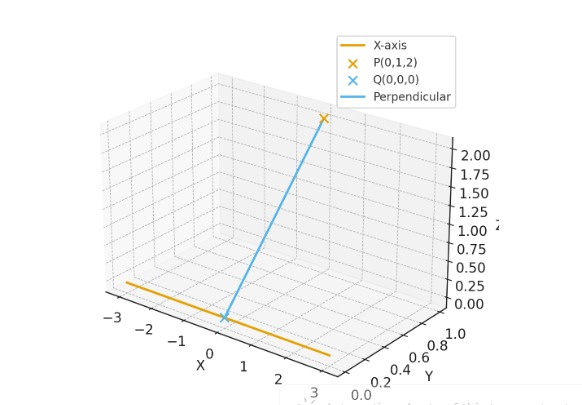
\includegraphics[width=0.75\linewidth]{figs/matgeo-4.8.35.jpeg}
    \caption{Perpendicular from $\vec{P}=\myvec{0\\1\\2}$ to thethe $x\text{-axis}$
 with foot $\vec{Q}=\myvec{0\\0\\0}$.}
    \label{fig:4.8.35-3d}
\end{figure}
\end{frame}

\end{document}
